\documentclass[12pt]{article}
\usepackage[utf8]{inputenc}
\usepackage{latexsym,amsfonts,amssymb,amsthm,amsmath,tikz,pgfplots,pdfpages,graphicx}
\usepackage{tikz}
\usepackage{url}
\usepackage{setspace}
\usepackage{csvsimple}
\usepackage{enumitem}
\usepackage{float}
\usepackage[document]{ragged2e}
\restylefloat{table}
\doublespacing
\setlength{\parindent}{0in}
\setlength{\oddsidemargin}{0in}
\setlength{\textwidth}{6.7in}
\setlength{\textheight}{9in}
\setlength{\topmargin}{0in}
\setlength{\headheight}{5pt}


\title{Report on Sentiment Analysis of Named Entities Taken From Live RSS News Feeds} 
\author{Ziyu Qiu, B00791470 \\ Cooper Gagnon, B00767631 \\ Matthew Moore, B00767194}

\begin{document}

\maketitle

\begin{center}
    \section*{Abstract}
    Record average sentiment of given named entities within a large custom news dataset. This custom dataset will be created from scraping several thousand news RSS feeds. Research how sentiment of named entities changes overtime. \\
\end{center}
\newpage
\section{Introduction}
\setlength{\parindent}{5ex}
Our ultimate goal of this project is to create a user interface where users can search for, and view sentiments of named entities overtime. We want to source this data from RSS feeds we have scraped ourself. As for an existing dataset, we had planned to use a data set containing 1 million news headlines \cite{Kaggle}. However, we found it much more engaging if we were to use real, and live data. As for an NLP model, we realized that we could use the pre-trained model provided by the python NLTK library. \\

\section{Related Work}
\hspace{\parindent} In the realm of natural language processing there has been a great amount of work done regarding the topic of sentiment analysis. This works stretches throughout multiple languages and data sources. 

One paper which relates directly to our topic is a paper from Tsinghua University on the Sentiment Analysis of Named Entities \cite{Wangx}. The authors of this report conducted a named entity filtration and sentiment analysis of a Chinese website, similar to Twitter. In the paper they incorporated and described methods for sentence segmentation, tokenisation, and `part of speech' (POS) tagging, much like what were able to accomplish with using the NLTK python library. 

Another paper, related to our work, was written at the Savitribai Phule Pune University, in India \cite{Sahayakv}. This paper outlines the process of performing sentiment analysis on Twitter data. The paper outlines multiple methods for performing the sentiment analysis such as Naive Bayes, Maximum Entropy, and Support Vector Machines, which are all widely used techniques for performing this type of analysis. This is very similar to the objective of our project as Twitter, much like news articles, is the voice of some public opinion on a topic. Our project differs as we are analyzing the effect that major news corporations may be projecting onto the public, where Twitter is mainly the voice of the general public. 

These methods aim to perform sentiment analysis using machine learning techniques, such as Naive Bayes models and support vector machines, to create and train their own models. Our method is different in that we are utilizing "VADER: A Parsimonious Rule-based Model" \cite{Hutto}, which is a part of the NLTK python library \cite{Sentiment}. The reason we have chosen this over classical models is that this is a method which provides us with a much more efficient classifier. This provides us with a "human-curated gold standard sentiment lexicon"\cite{Hutto}, a model which does not suffer from a speed-performance trade-off, which is perfect for analyzing live data. As well, this alternative model provides us with an intensity score of the sentiment, instead of a simple positive or negative tag, which provides us with the ability to visualize the change in opinion over time, and the intensity of the sentiment emotion for a particular named entity.

\section{Problem Definition and Methodology}
\hspace{\parindent} The mass media, and especially news corporations, often thrive off of the emotions of the general public. The creation of riveting news headlines are used to draw in an audience, often times with great exaggeration and biased opinion. One of the issues which arises from this is the subconscious control of ones opinion due to the opinion of another, which in this instance are news corporations. The goal of our project is to create an application which can help the public understand the influence of the media on our perception of ideas and topics. 

Our idea was to gather as much information as possible and find a way to display this information in a meaningful, and easy to understand way. We began gathering information by scraping RSS feeds for news headlines. We stored these headlines in a MySQL database, along with other informatiOur initial on such as the date it was gathered. experimentation consisted of querying a fixed amount of information from the database and testing natural language processing techniques on the data such as named entity extraction with the python NLTK toolkit. We were able to extract the sentiment of the original sentence, and from there we would associate each named-entity with that sentiment. This would allow us to analyze the sentiment associated with certain topics, ideas, named, etc. 

\section{Custom Dataset Creation}
\hspace{\parindent}In order to create a custom dataset for this implementation we gathered over 2000 RSS feeds, to scrape and store in MySQL\@. We scraped the RSS feeds for the title and dates, which were then stored. We began with a large collection of new websites used by Google to produce their news section \cite{GoogleNewsBlog}. Selecting only the English websites, we scraped their html to find their RSS feed. We then inserted all the functioning RSS feeds into a MySQL database which we scraped daily.

Overall, we were able to gather over three hundred thousand samples of news titles as of writing this report. Each RSS feed represents a news corporation of some sort, some samples may be bias in one direction while others are opposite. Ultimately this allows for an average across different opinions and sources, which we wanted to extend in either direction as much as possible. As well, all sample feeds were sourced in English. Creating our own dataset allows us to update the data in real time.

 Figure~\ref{RSS} shows an example of some RSS feeds from our database. As shown, there is a great variety of news sources, and types that we are gathering. Even though all of the sources are in English, many of the sources are from countries outside of Canada and the USA. 

\vspace*{20px}

\begin{figure}[htp]
    \centering
    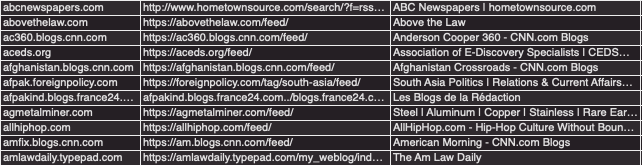
\includegraphics[scale=0.7]{feeds.PNG} \\
    \caption{RSS Feeds}
    \label{RSS}
\end{figure}





\clearpage
\section{Experiments}
\subsection{Experiment Environment Introduction}

We created a simple user interface in order to be able to properly display this information to the general public, as seen below. We built these user interfaces using Bootstrap\cite{Bootstrap}, Google charts\cite{GoogleChart} and jQuery\cite{jQuery}.

\begin{figure}[htp]
    \centering
    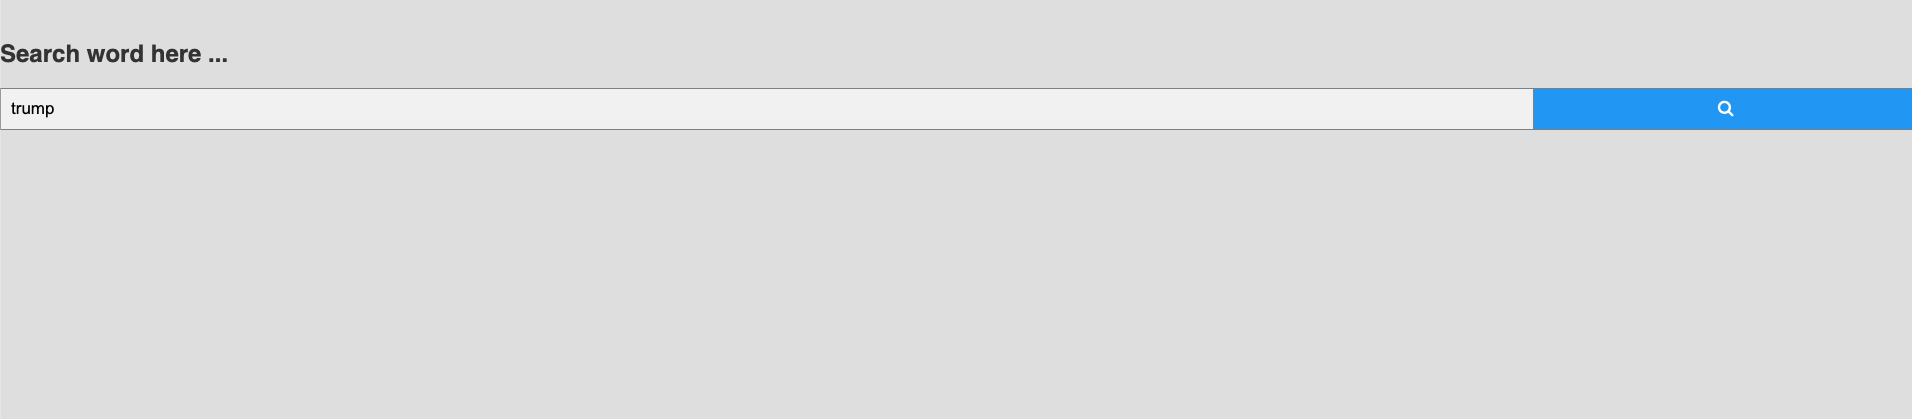
\includegraphics[scale=0.25]{main.PNG} \\
    \caption{Search Page}
\end{figure}


\begin{figure}[htp]
    \centering
    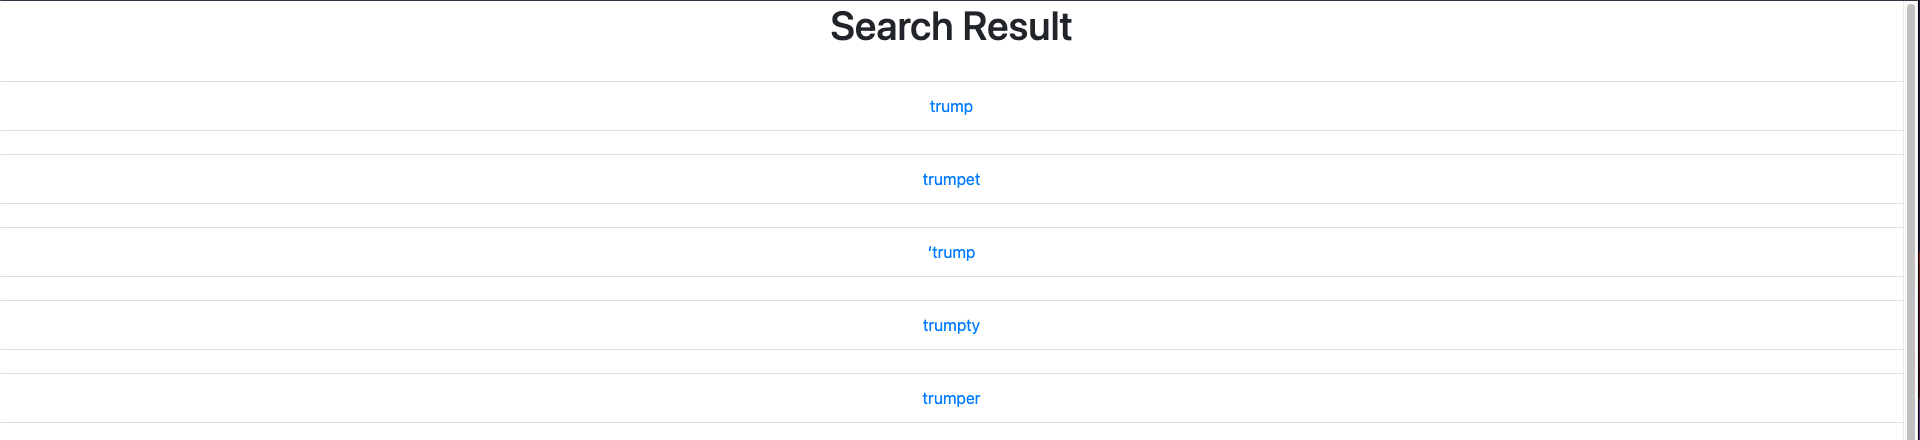
\includegraphics[scale=0.25]{list.PNG} \\
     \caption{Results Page}
\end{figure}


\begin{figure}[htp]
    \centering
    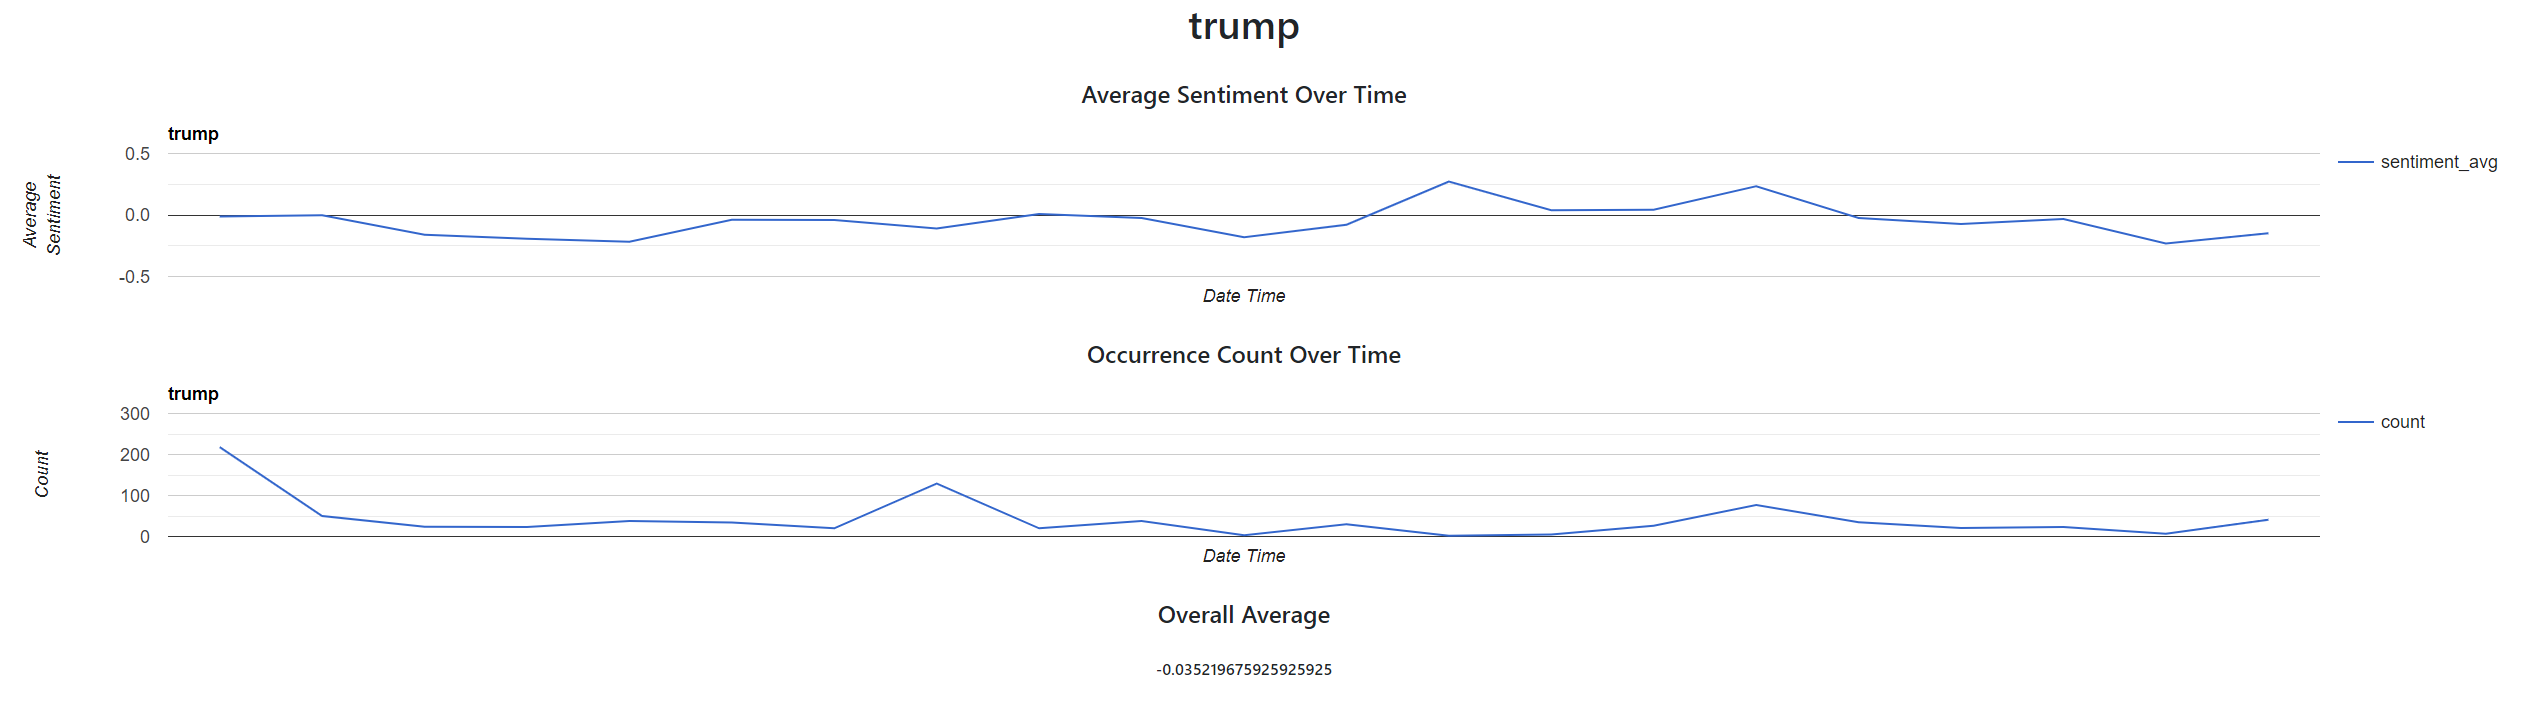
\includegraphics[scale=0.25]{trump.PNG} \\
    \caption{Graph Page}
\end{figure}


\subsection{Experimental Setup}
\hspace{\parindent}  We began by taking small sub-samples of the data which we would chunk, and extract the named entities from. From there we would take the original sample news headline and perform sentiment analysis on the text, using the `VADER Sentiment Intensity Analyzer' function from the python NLTK\@. We were able record the amount of times a sentence included a given named entity, as well as a sum of the sentiments that were calculated. This allowed us to divide the sum of sentiments by the count of occurrences, which provided us with an overall average.

After conducting some small scale experiments we moved onto processing the entirety of the data, on a `day by day' basis. For each day, we were able to calculate the average sentiment. This allowed us to see how the sentiment trend progressed over time. Ultimately, this would be the data that would become beneficial to our graph and user interface, which would allow anyone to visualize this data. 

Once we had established a successful method, we were able to run our data collection script on a timer. We have one script which gathers RSS feed data and populates the news headline database, and another script that runs once a day which extract the named entities, and sentiment data. This allows our application to operate in real time, allowing our interface to display new relevant data every day. Ultimately this is to ensure that any member of the general public can understand, and visualize the influence of the media on certain topics. Not only can one see known and distinguished topics, one can also see currently relevant and new topics.

\clearpage

\subsection{Examples}

\hspace{\parindent} Example of Named Entity Table.
\begin{table}[H]
    \begin{tabular}{|l|l|l|l|l|l|l|l|}
        \hline
        id & named\_entity & sentiment & update & date & count    \\ \hline
        58             & pipeline       & 0.4215       & 2021-02-26 00:00:00       & 2021-02-26 00:00:00       & 1       \\ \hline
        59             & genfit       & -0.0258       & 2021-02-26 00:00:00       & 2021-02-26 00:00:00       & 1             \\ \hline
        60             & pfizer       & -0.1341       & 2021-02-26 00:00:00       & 2021-02-26 00:00:00       & 2        \\ \hline
        61            & china       & -0.6597       & 2021-02-26 00:00:00       & 2021-02-26 00:00:00       & 1       \\ \hline
    \end{tabular}
\end{table}


Example of News Data Table.
\begin{table}[H]
    \begin{tabular}{|l|l|l|l|l|l|l|l|}
        \hline
        id & title  \\ \hline
        279    & Lebanon, France ink 3 defense agreements     \\ \hline
        280            & Germany convicts Syrian regime officer of crimes against humanity       \\ \hline
        281           & Hunger in Central America skyrockets, U.N. agency says             \\ \hline
        282           & More power blackouts await Lebanon. Energy ministry will soon run out fuel        \\ \hline
    \end{tabular}
\end{table}

\clearpage

\section{Results and Discussion}
Our application proved to be very useful for displaying the influence of the media in an easy to understand and visual way. The NLP techniques and concepts we used were able to extract important information, such as named-entities, and the sentiment of the sentence, and combine both into a graph format, which can be understood by anyone who is unfamiliar with the technicalities. For instance, as seen in Figure~\ref{suez}, one can see how there was a spike near March 28th, 2021, when a highly notable event took place. This was the time when a ship was stuck in the canal, and one can see not only the number of times `suez' was mentioned, but the influence on sentiment associated with it.

\begin{figure}[htp]
    	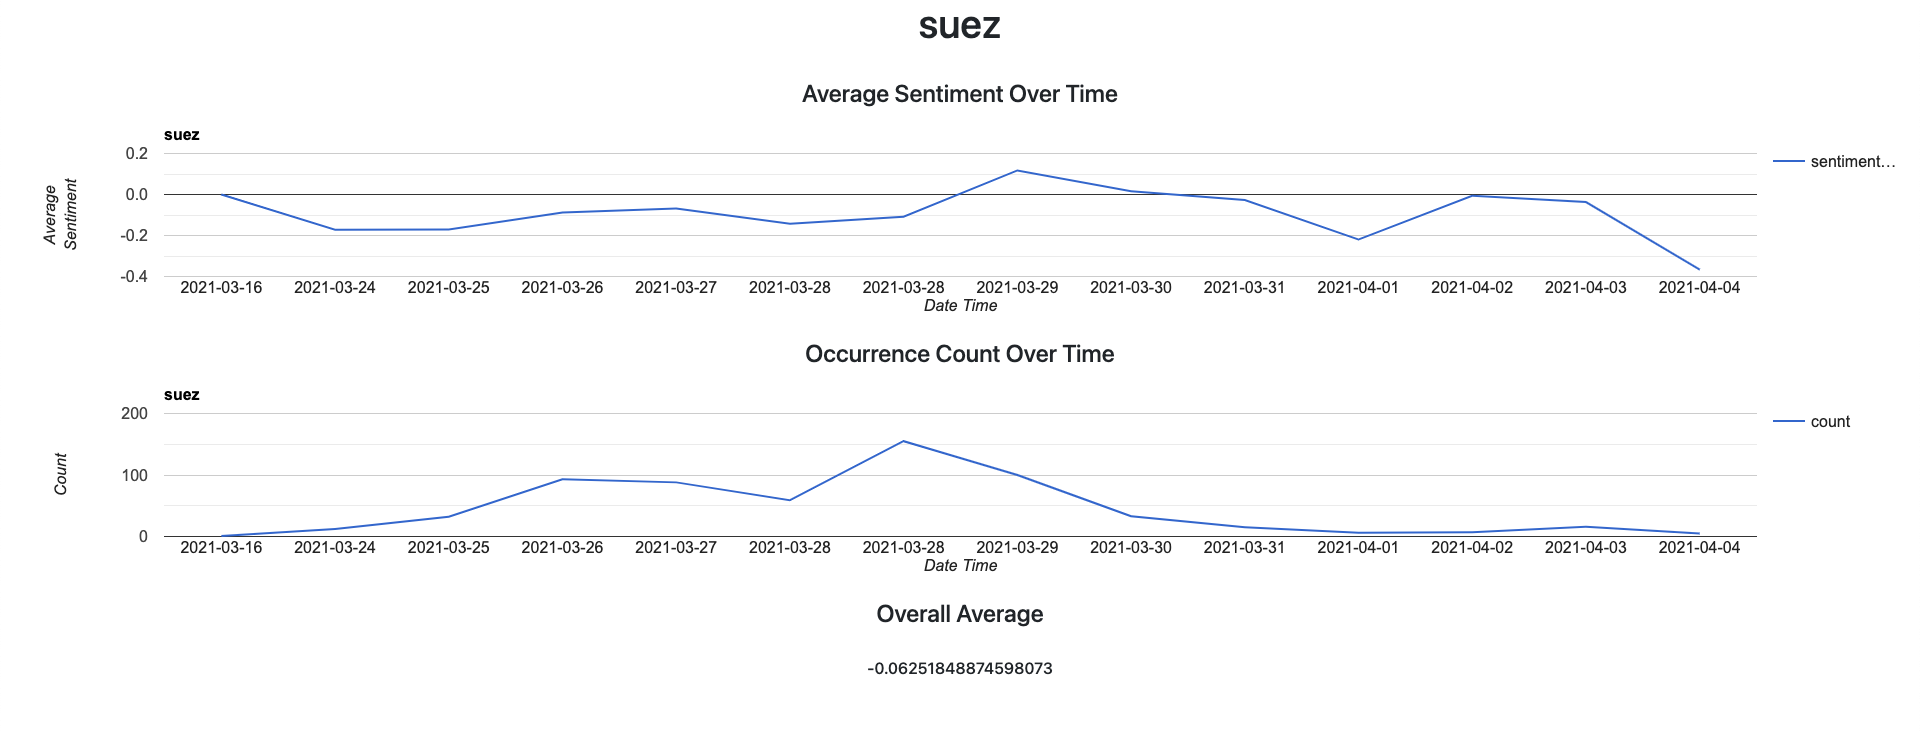
\includegraphics[scale=0.25]{suez.PNG} \\
	\caption{'suez'}
	\label{suez}
\end{figure}

Among our tests, we found another interesting example. The recent rise and fall of gamestop's stock, which is a popular topic, matched our analysis to a large extent. Gamestop is a video games retailer, but recently due to a Reddit Forum called "WallStreetBets", a lot of users start to bet on its stock. So in the recent months, whenever the name gamestop shows on the media, it mostly represents the stock instead of the retailer itself. The gamestop stock ticker is 'GMR'. We can see from the two tables below that there is a great synchronization between the ups and downs of these two tables (Gamestop Sentiment: Figure~\ref{gamestop-sentiment}, Gamestop stock: Figure~\ref{gamestop-stock}).

\begin{figure}[htp]
    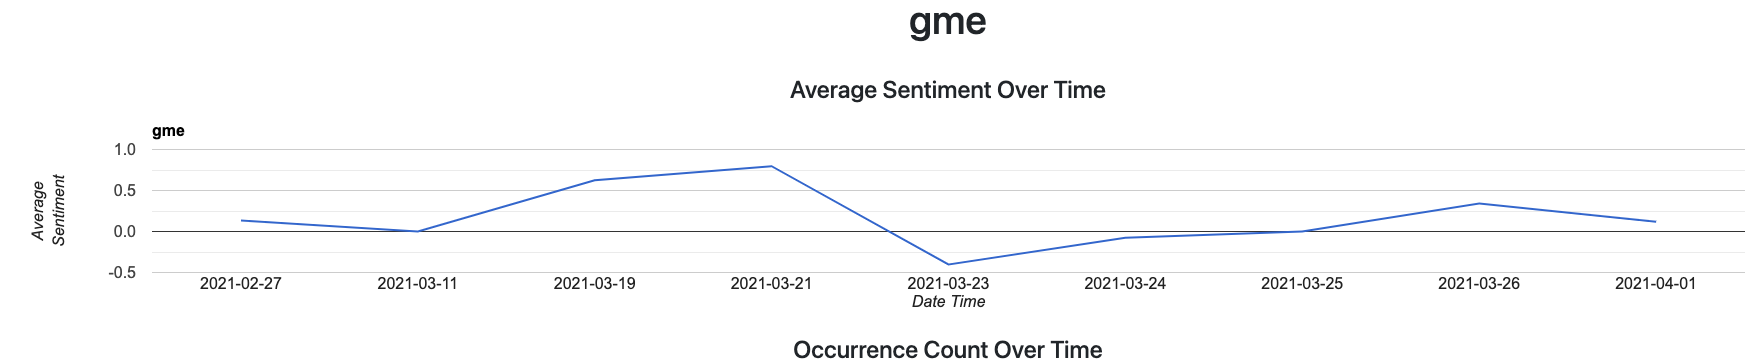
\includegraphics[scale=0.25]{gamestop-avg.PNG} \\
\caption{Gamestop sentiment over time}
\label{gamestop-sentiment}
\end{figure}

\begin{figure}[htp]
    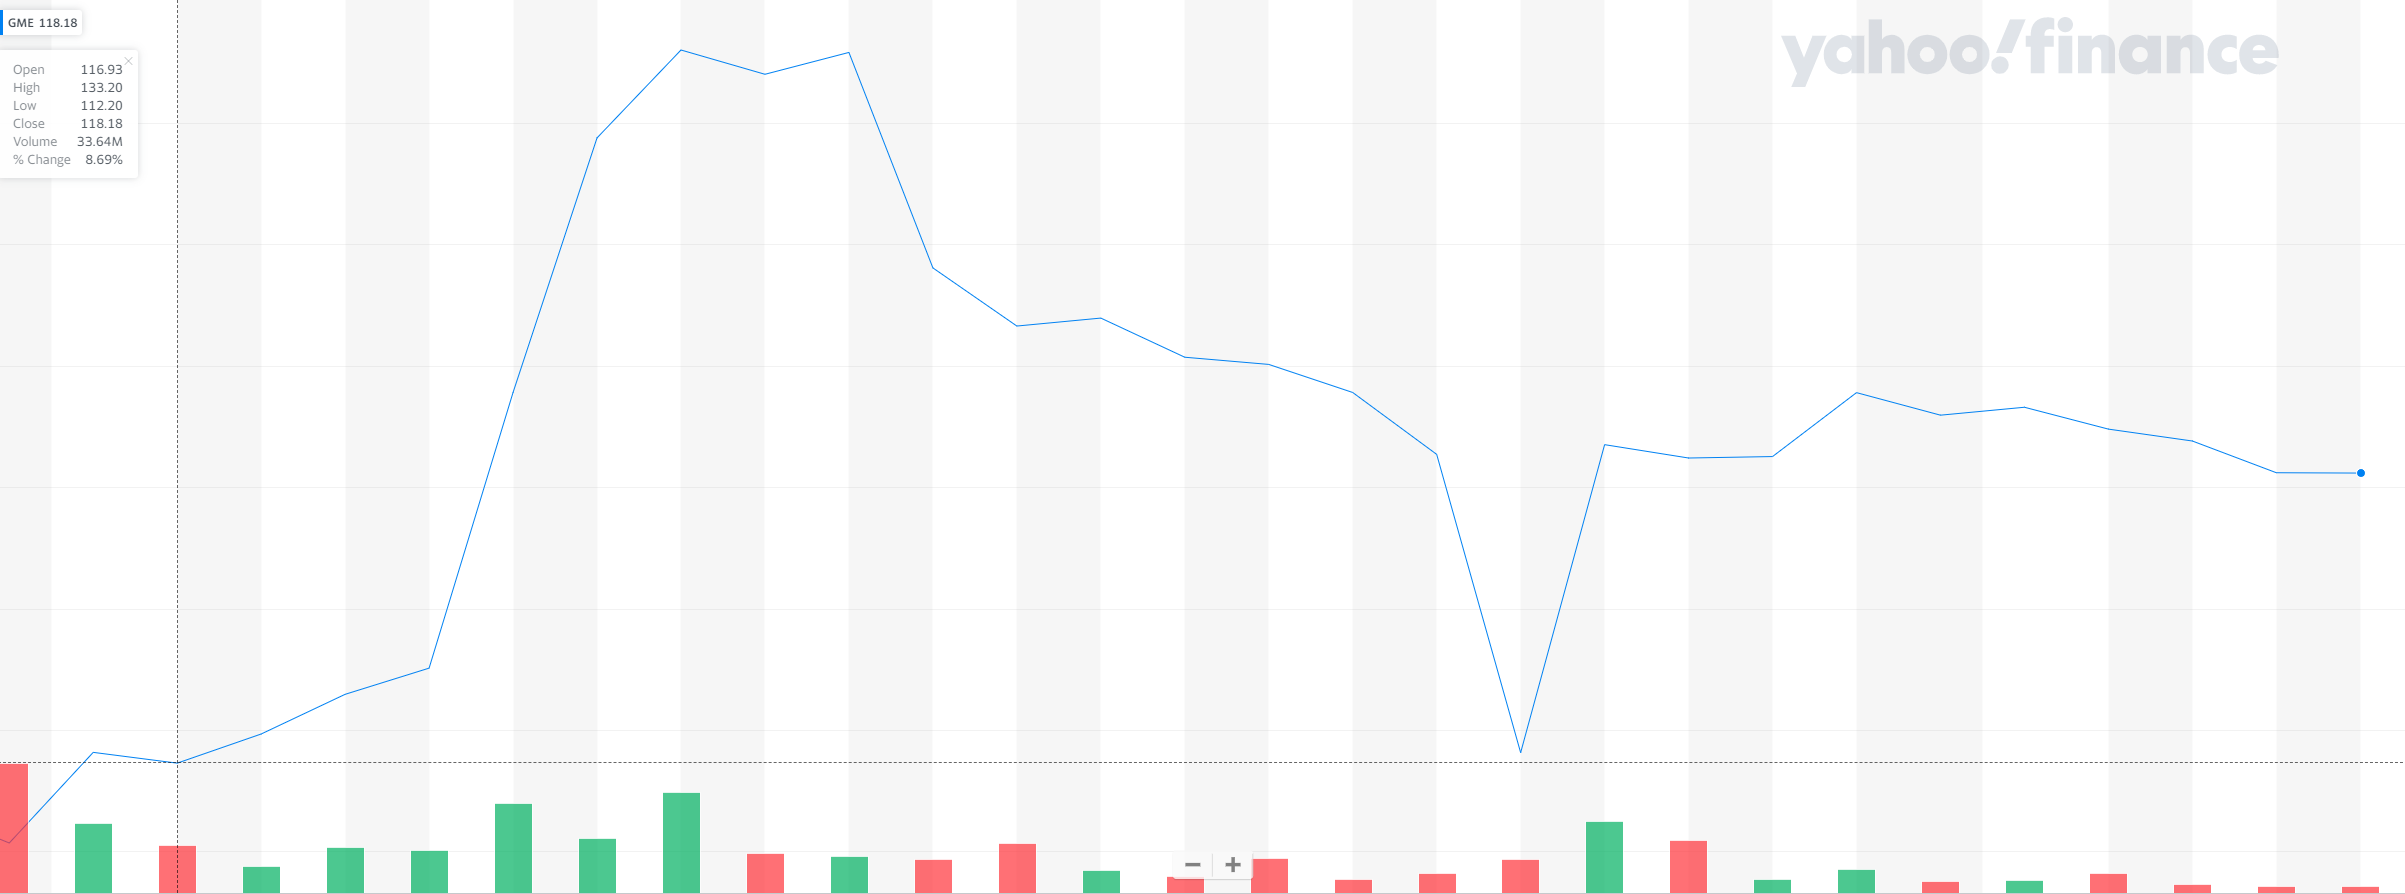
\includegraphics[scale=0.25]{gme-stock.PNG} \\
	\caption{Gamestop stock value over time \cite{Yahoo}}
\label{gamestop-stock}
\end{figure}


\section{Conclusion and Outlook}

In conclusion our methods of determining the average sentiment of a named entity overtime proved to be very successful. The custom dataset came together very well as we were able to collect over 2000 RSS feeds as our news sources, and then collect over 399,000 samples of news titles over the span of a month and a half of recording. From this we extracted over 200,000 unique named entities. All of which were available for users to search and view graphs of sentiment overtime using our user interface.

\clearpage
\section{Bibliography}
\begin{thebibliography}{10}

\bibitem{GoogleNewsBlog} Agarwal Amit, `Which Sites and Blogs are Indexed by Google News?', July. 2011 \url{https://www.labnol.org/internet/sites-indexed-in-google-news/19323/}

\bibitem{Bootstrap} Bootstrap \url{https://getbootstrap.com/}

\bibitem{GoogleChart} Google Chart \url{https://developers.google.com/chart/}

\bibitem{Hutto} Hutto, C.J. \& Gilbert, E.E. (2014). VADER: A Parsimonious Rule-based Model for Sentiment Analysis of Social Media Text. Eighth International Conference on Weblogs and Social Media (ICWSM-14). Ann Arbor, MI, June 2014.

\bibitem{jQuery} jQuery \url{https://jquery.com/}

\bibitem{Kaggle} Kulkarni Rohit `A Million News Headlines' Kaggle, Feb. 2021, \url{https://www.kaggle.com/therohk/million-headlines}

\bibitem{Sahayakv} Sahayak, Varsha, et al. Sentiment Analysis on Twitter Data. Savitribai Phule Pune University, India, Jan. 2015

\bibitem{Sentiment} Sentiment Analysis \url{https://www.nltk.org/howto/sentiment.html}

\bibitem{Wangx} Wang, Xinzhi, et al. Sentiment Analysis of Name Entity for Text.

\bibitem{Yahoo} Yahoo Finance \url{https://ca.finance.yahoo.com/}

\end{thebibliography}

\end{document}
